\documentclass{article}

\usepackage[polish]{babel}
\usepackage{minted}
\usepackage[letterpaper,top=2cm,bottom=2cm,left=3cm,right=3cm,marginparwidth=1.75cm]{geometry}
\usepackage{amsmath}
\usepackage{graphicx}
\usepackage[colorlinks=true, allcolors=blue]{hyperref}
\usepackage[T1]{fontenc}
\usepackage[table,xcdraw]{xcolor}
\usepackage{float}
\usepackage[figurename=Wykres]{caption}
\definecolor{mategreen}{RGB}{102, 176, 50}

\title{MOwNiT - Zagadnienie interpolacji Hermite'a}
\author{Jakub Frączek}

\begin{document}

\maketitle

\section{Temat ćwiczenia}

\subsection{Przygotowanie}

Zagadnienie interpolacji:
Pprzygotować program wyznaczający wielomian interpolujący zgodnie ze wzorem Hermite'a.

W obu przypadkach węzły mogą być rozmieszczone:
\begin{itemize}
\item równomiernie w całym przedziale (uwzględniając końce przedziału),
\item zgodnie z zerami wielomianu Czebyszewa.
\end{itemize}

Przygotować program do wizualizacji wykresu funkcji zadanej określoną liczbą punktów lub określonym wzorem.

\subsection{Właściwe ćwiczenie}

1. Dla jednej z poniższych funkcji (podanej w zadaniu indywidualnym) wyznacz dla zagadnienia 
Hermite’a wielomian interpolujący.  
Interpolację przeprowadź dla różnej liczby węzłów (np. n = 3, 4, 5, 7, 10, 15, 20). Dla każdego 
przypadku interpolacji porównaj wyniki otrzymane dla różnego rozmieszczenia węzłów: 
równoodległe oraz Czebyszewa*. 
Oceń dokładność, z jaką wielomian przybliża zadaną funkcję.  
Poszukaj wielomianu, który najlepiej przybliża zadaną funkcję. 
Wyszukaj stopień wielomianu, dla którego można zauważyć efekt Runge’go (dla równomiernego 
rozmieszczenia węzłów). Porównaj z wyznaczonym wielomianem dla węzłów Czebyszewa.

\subsection{Funkcja dla której przeprowadzone zostało doświadczenie}

\begin{center}
\(f(x) = 10 * m + \frac{\mathrm{x}_{}^{2}}{k} - 10 * m * cos(k*x)\)
\end{center}

\noindent
gdzie:

\bigbreak

\(k = 1.5\)
\newline \indent
\(m = 3.0\)
\newline \indent
\(x \in [-4\pi, 4\pi]\)
\bigbreak
Wykres funkcji (wykres 1)

\begin{figure}[H]
  \centering
  \begin{minipage}[b]{0.3\textwidth}
    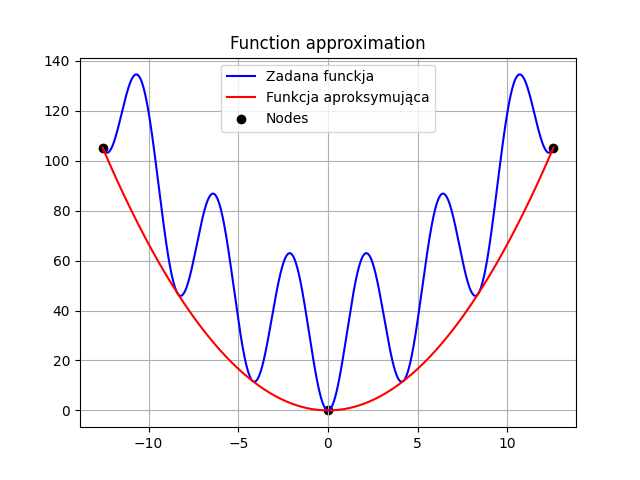
\includegraphics[width=\textwidth]{img01.png}
    \caption{Dana funkcja}
  \end{minipage}
\end{figure}

\subsection{Pochodna funkcji dla której przeprowadzone zostało doświadczenie }

Pochodna funkcji (wykres 2)

\begin{figure}[H]
  \centering
  \begin{minipage}[b]{0.3\textwidth}
    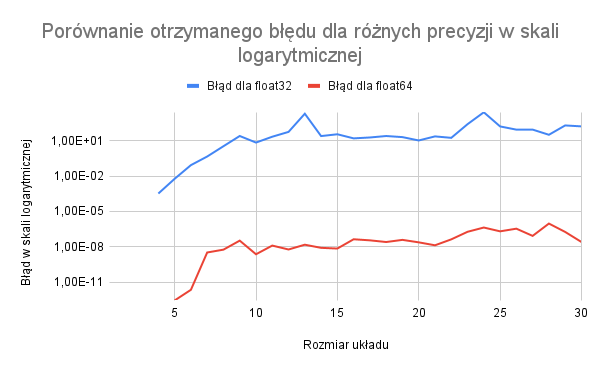
\includegraphics[width=\textwidth]{img02.png}
    \caption{Dana funkcja}
  \end{minipage}
\end{figure}

\section{Dane techniczne}

\subsection{Hardware}

Doświadczenie zostało przeprowadzone na komputerze z procesorem Intel Core i5-9300H 2.40 GHz oraz 32 GB pamięci RAM 2666 MHz.

\subsection{Software}

Wykorzystany został język Python w wersji 3.11.8 wraz z bibliotekami:
\begin{itemize}
\item math
\item copy
\item matplotlib
\item numpy
\end{itemize}

\section{Iterpolacja Hermite'a}

Wielomian interpolacyjny Hermite'a można wyrazić wzorem

\[\mathrm{H}_{n}^{}(x) = \sum_{i = 0}^{n}\mathrm{b}_{l}^{}\mathrm{p}_{l}^{}(x) = 
\sum_{i = 0}^{k}\sum_{j=0}^{\mathrm{m}_{i}^{} - 1}\mathrm{b}_{(s(i) + j)}^{} \cdot 
\mathrm{p}_{s(i) + j}^{}(x) \]

\noindent
gdzie:

\bigbreak

\(\mathrm{p}_{s(0)}^{}(x) = 1\) 

\indent

\(\mathrm{p}_{s(i) + j}^{}(x) = \mathrm{(\mathrm{x - \mathrm{x}_{0}^{}}_{}^{})}_{}^{\mathrm{m}_{0}^{}}
\mathrm{(\mathrm{x - \mathrm{x}_{1}^{}}_{}^{})}_{}^{\mathrm{m}_{1}^{}}...
\mathrm{(\mathrm{x - \mathrm{x}_{i - 1}^{}}_{}^{})}_{}^{\mathrm{m}_{i-1}^{}}
\mathrm{(\mathrm{x - \mathrm{x}_{i}^{}}_{}^{})}_{}^{\mathrm{j}_{}^{}}\)

\indent

\(
s(i) = 
\begin{cases}
    0 & \text{dla } i = 0 \\
    \mathrm{m}_{0}^{} + \mathrm{m}_{1}^{} + ... + \mathrm{m}_{i - 1}^{} & \text{dla } i > 0
\end{cases}
\)

\indent

\(i = 0, 1, ..., k\)

\indent

\(j = 0,1,...,\mathrm{m}_{i}^{} - 1\)

\indent

Współczynniki \(\mathrm{b}_{l}^{}\) to kolejne ilorazy różnicowe.

\section{Metody szacowania błędu przybliżenia funkcji}

\subsection{Największa różnica wartości funkcji}

Największa różnica między wartością funkcji interpolowanej, a funkcji interpolującej:

\begin{center}
    \(\max_{x\in [a, b]} |F(x) - \mathrm{P}_{n}^{}(x)|\)
\end{center}

\subsection{Błąd średniokwadratowy}

Suma kwadratów różnic mięcy wartością funkcji interpolowanej, a funkcji interpolującej podzielona przez ilość punktów, w których wykonujemy porównanie:

\begin{center}
\(\frac{1}{N} * \sum_{i = 1}^{N}\mathrm{(F(\mathrm{x}_{i}^{}) - \mathrm{P}_{n}^{}(\mathrm{x}_{i}^{}))}_{}^{2}\)
\end{center}

Jak zostało również zaznaczone poniżej, w tym ćwiczeniu do wyznaczania błędów korzystam z 1000 równoodległych punktów, zatem w tym przypadku \(N = 1000\).

\section{Wyniki}

Błędy zostały policzone z wykorzystaniem 1000 równoodlegle wygenerowanych punktów.

\subsection{Błąd maksymalny dla węzłów z zakresu [3, 30]}

W tym przypadku, jak pokazano na wykresie 3 i 4, dla liczby wężłów od 7 do 12 efekt Rungego był największy. Widać także, że błąd zaczyna maleć do 16 / 21 węzła. Widać także, że korzystając z węzłów Czebyszewa do 20 węzła można średnio otrzymać dużo mniejszy błąd niż korzystając z węzłów równoodległych.

\begin{figure}[H]
  \begin{minipage}[b]{0.49\textwidth}
    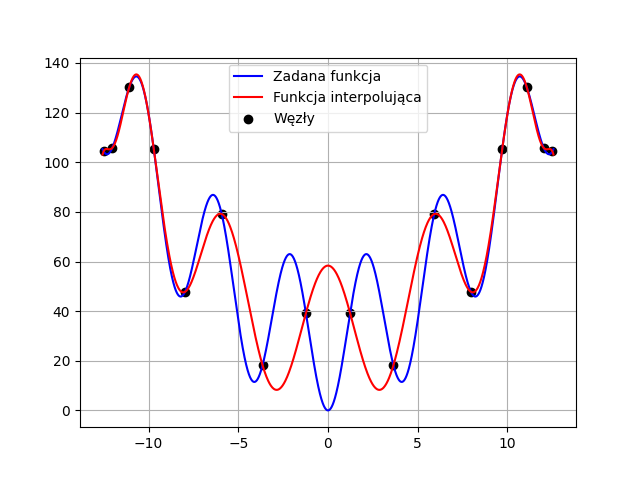
\includegraphics[width=\textwidth]{img03.png}
    \caption{Błąd maksymalny}
  \end{minipage}
  \hfill
  \begin{minipage}[b]{0.49\textwidth}
    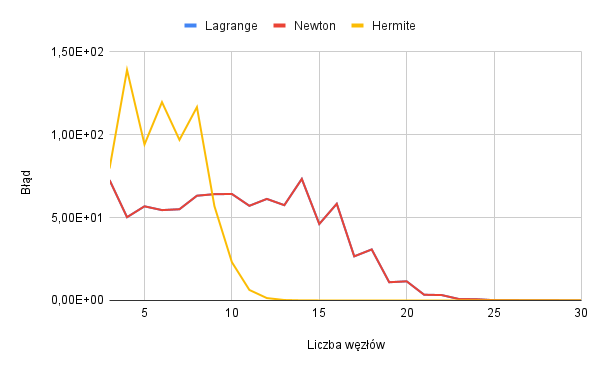
\includegraphics[width=\textwidth]{img04.png}
    \caption{Błąd w skali logarytmicznej}
  \end{minipage}
\end{figure}

\subsection{Błąd maksymalny dla węzłów z zakresu [31, 50]}

Jak widać na wykresach 5 i 6 od 30 węzła błąd zaczyna konsekwentnie rosnąć, a już dla 50 węzłów jest on ogromny. Można zauważyć także, że błąd dla węzłów Czebyszewa rośnie szybciej od błędu dla węzłów równoodległych. Zaobserwowany błąd nie wynika już z efektu Rungego, a z niedokładności zapisu liczb zmiennoprzecinkowych w komputerze, co implikuje niedokładne operacje na tych liczbach oraz brak możliwości zapisania każdej możliwej wartości co skutkuje zaokrągleniami i w dużej skali, tak jak tutaj już jest to bardzo widoczne i uniemożliwia precyzyjne przybliżenie zadanej funkcji.

\begin{figure}[H]
  \begin{minipage}[b]{0.49\textwidth}
    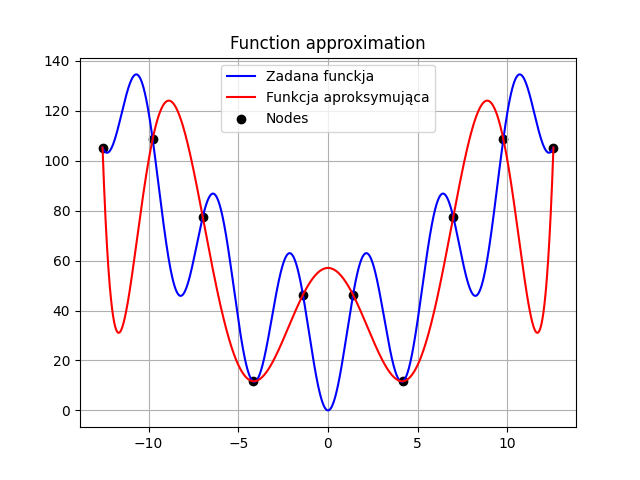
\includegraphics[width=\textwidth]{img05.png}
    \caption{Błąd maksymalny}
  \end{minipage}
  \hfill
  \begin{minipage}[b]{0.49\textwidth}
    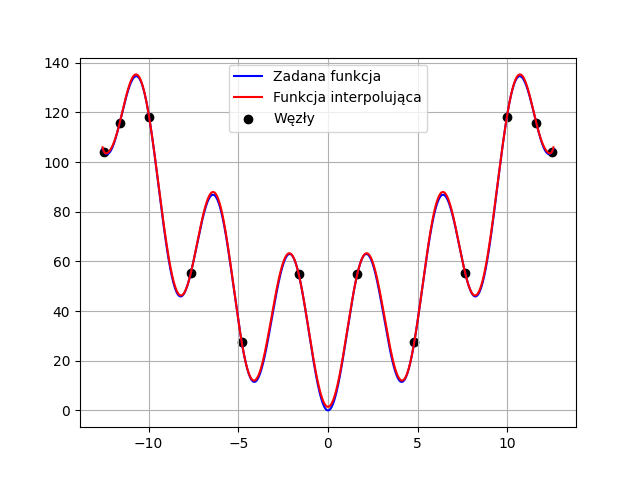
\includegraphics[width=\textwidth]{img06.png}
    \caption{Błąd w skali logarytmicznej}
  \end{minipage}
\end{figure}

\subsection{Błąd średniokwadratowy dla węzłów z zakresu [3, 30]}

Podobnie jak dla błędu maksymalnego, średio błąd dla węzłów czebyszewa jest mniejszy do 20 wężła, potem sytuacja się odwraca co widać na wykresie 8 oraz można zaobserować "peak" efektu Rungego od 7 do 12 węzła (wykres 7).

\begin{figure}[H]
  \begin{minipage}[b]{0.49\textwidth}
    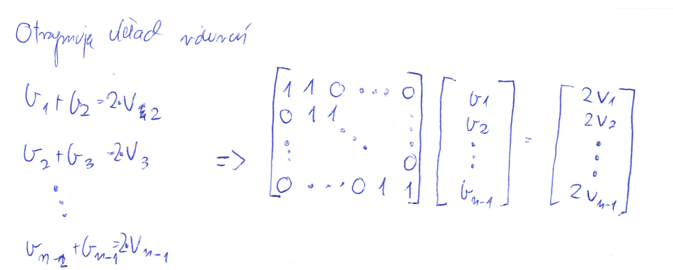
\includegraphics[width=\textwidth]{img07.png}
    \caption{Błąd średniokwadratowy}
  \end{minipage}
  \hfill
  \begin{minipage}[b]{0.49\textwidth}
    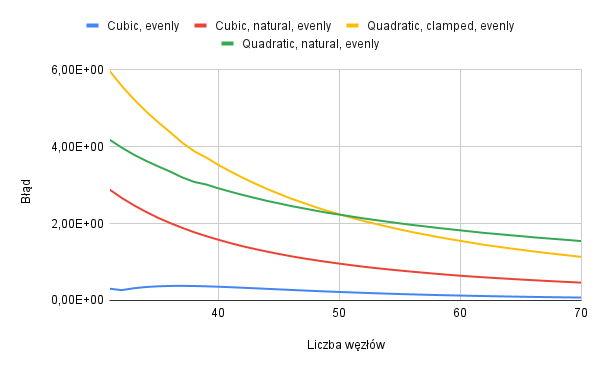
\includegraphics[width=\textwidth]{img08.png}
    \caption{Błąd w skali logarytmicznej}
  \end{minipage}
\end{figure}

\subsection{Błąd średniokwadratowy dla węzłów z zakresu [31, 50]}

Sytuacja jest taka sama jak dla błędu maksymalnego.Jak widać na wykresach 9 i 10 od 30 węzła wartości błędów zaczynają powoli rosnąć i szybko osiągają nieakceptowany przy przybliżeniu pułap. Błąd dla węzłów Czebyszewa jest w tym przedziale większy niż dla węzłów równoodległych.

\begin{figure}[H]
  \begin{minipage}[b]{0.49\textwidth}
    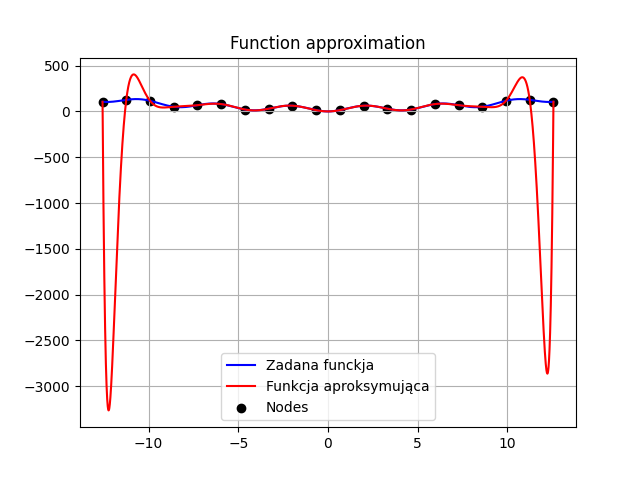
\includegraphics[width=\textwidth]{img09.png}
    \caption{Błąd średniokwadratowy}
  \end{minipage}
  \hfill
  \begin{minipage}[b]{0.49\textwidth}
    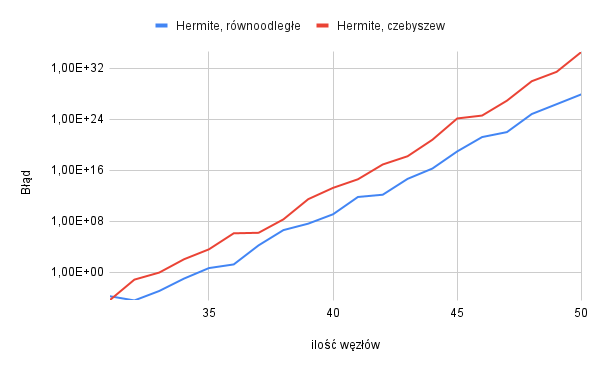
\includegraphics[width=\textwidth]{img10.png}
    \caption{Błąd w skali logarytmicznej}
  \end{minipage}
\end{figure}

\subsection{Efekt Rungego}

"Peak" efektu Rungego zachodzi dla 8 równoodległych węzłów, co zostało zaprezentowane na wykresie 11. Jak widać w najbardziej oddalonym punkcjia błąd wynosi aż ponad 1000. Następnie znaczyna zanikać, aż do 21 węzła, dla którego otrzymujemy najlepsze przybliżenie metodą równoodległych węzłów.

\begin{figure}[H]
  \centering
  \begin{minipage}[b]{0.93\textwidth}
    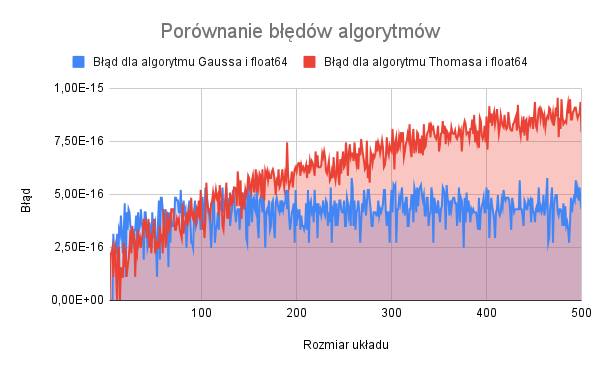
\includegraphics[width=\textwidth]{img13.png}
    \caption{Dana funkcja}
  \end{minipage}
\end{figure}



\subsection{Najlepsze przybliżenie interpolowanej funkcji}

Najlepszym przybliżeniem ze względu na największą rónicę wartości była interpolacja z wykorzystaniem 19 węzłów czebyszewa (wykres 12), a ze względu na błąd średniokwadratowy interpolacja z wykorzystaniem 23 równoodległych węzłów (wykres 13).

\begin{figure}[H]
  \begin{minipage}[b]{0.49\textwidth}
    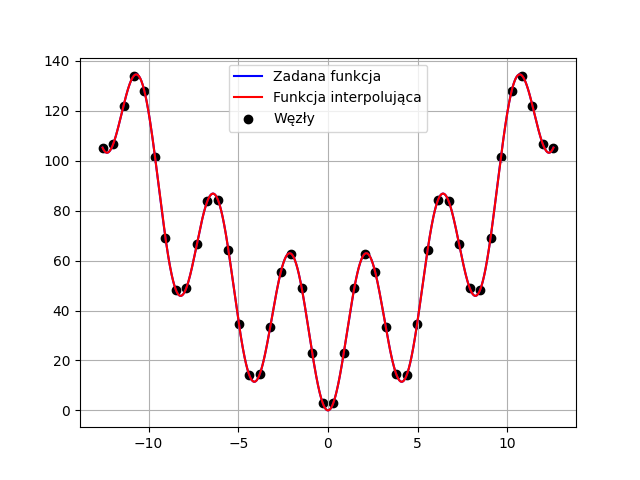
\includegraphics[width=\textwidth]{img11.png}
    \caption{Interpolacja z 19 w. Czebyszewa}
  \end{minipage}
  \hfill
  \begin{minipage}[b]{0.49\textwidth}
    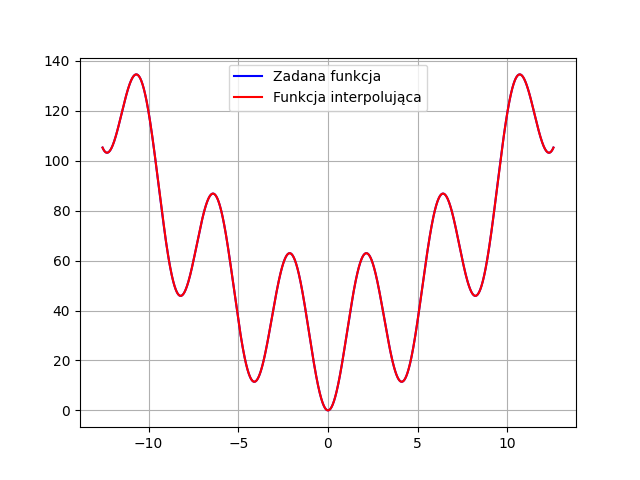
\includegraphics[width=\textwidth]{img12.png}
    \caption{Interpolacja z 23 równoodległych w.}
  \end{minipage}
\end{figure}

Poniżej w tabli 1 oraz 2 znajdują się wartośći najmniejszych otrzymanych błędów dla dwóch różnych sposobów wyboru węzłów. Na zielono zaznaczonea jest wartość namniejsza dla danego typu błędu i sposobu doboru węzłów, a obok dla porównania znajduje się wartość otrzymana alternatywnym sposobem generacji węzłów. Warto zauważyć, że nie ma między tymy wartościami ogromnej różnicy, a otrzymane błędy są dość małe.

\begin{table}[!ht]
    \centering
    \begin{tabular}{|l|l|l|}
    \hline
        ilość węzłów & Hermite, równoodległe & Hermite, czebyszew  \\ \hline
        19 & 5,81E-03 & \textcolor{mategreen}{7,92E-04}  \\ \hline
        21 &  \textcolor{mategreen}{4,61E-04} & 2,04E-03 \\ \hline
    \end{tabular}
    \caption{Prównanie błędu maksymalnego dla najmniejszych otrzymanych błędów}
\end{table}

\begin{table}[!ht]
    \centering
    \begin{tabular}{|l|l|l|}
    \hline
        ilość węzłów & Hermite, równoodległe & Hermite, czebyszew  \\ \hline
        19 & 1,05E-06 & \textcolor{mategreen}{4,46E-09}  \\ \hline
        23 & \textcolor{mategreen}{8,54E-09} & 1,77E-07 \\ \hline
    \end{tabular}
    \caption{Prównanie błędu średniokwadratowego dla najmniejszych otrzymanych błędów}
\end{table}

\subsection{Porównanie warości błędu maksymalnego dla wybranej liczby węzłów}

Jak można zobaczyć w tabli 3, zachodzi drasyczna różnica pomiędzy błędem dla 40, a 50 węzłów. 

\begin{table}[!ht]
    \centering
    \begin{tabular}{|l|l|l|}
    \hline
        ilość węzłów & Hermite, równoodległe & Hermite, czebyszew  \\ \hline
        10 & 1,01E+03 & 2,31E+01  \\ \hline
        20 & 1,03E-03 & 1,56E-03  \\ \hline
        30 & 3,33E-02 & 5,43E-02  \\ \hline
        40 & 7,16E+05 & 5,22E+07  \\ \hline
        50 & 2,09E+15 & 3,47E+18 \\ \hline
    \end{tabular}
    \caption{Prównanie błędu maksymalnego dla wybranej liczby węzłów}
\end{table}

\subsection{Porównanie warości błędu średniokwadratowego dla wybranej liczby węzłów}

Podobnie jak powyżej tabela 4 pokazuje ogromną różnicę błędów pomiędzy 40, a 50 węzłem.

\begin{table}[!ht]
    \centering
    \begin{tabular}{|l|l|l|}
    \hline
        ilość węzłów & Hermite, równoodległe & Hermite, czebyszew  \\ \hline
        10 & 7,43E+04 & 9,75E+01  \\ \hline
        20 & 1,75E-08 & 1,29E-08  \\ \hline
        30 & 1,87E-05 & 2,00E-05  \\ \hline
        40 & 1,20E+09 & 1,70E+13  \\ \hline
        50 & 8,65E+27 & 4,01E+34 \\ \hline
    \end{tabular}
    \caption{Prównanie błędu średniokwadratowego dla wybranej liczby węzłów}
\end{table}

\section{Wnioski}

\begin{itemize}
\item Dla małej ilości węzłów (do 20) lepsze przybliżenie funkcji dają węzły Czebyszewa
\item Błąd maksymalny pozwala trafnie określić, gdzie zachodzi efekt Rungego (dla małej ilości węzłów). Dla dużej ilości węzłów bardzo widoczny jest problem z reprezentacją liczb zmiennoprzecinkowych w komputerze, ponieważ otrzmane wartości błędów są ogromne
\item Iterpolacja Hermite'a daje dobre przybliżenie dla odpowiednio dobranej liczby węzłów.
\end{itemize}

\end{document}
